\documentclass{article}

\usepackage{amsmath}
\usepackage{booktabs}
\usepackage[labelfont=bf]{caption}
\usepackage{subcaption}
\usepackage[top=1in,bottom=1in]{geometry}
\usepackage{float}
\usepackage{pgfplots}
\usepackage{pgfplotstable}
\usepackage{tikz}

\pgfplotsset{compat=1.18}
\usepgfplotslibrary{statistics}

\author{Henry Oehlrich \and Lahari Jaligama}
\title{Difference between mean typing speeds of STEM and humanities students}

\begin{document}
\maketitle{}

\section{Question, Hypothesis, \& Data Collection}

Is there a statistically significant difference between the mean typing speed
for students who consider themselves more STEM-oriented and those who consider
themselves more humanities-oriented?

\begin{gather}
    H_0: \overline{STEM} = \overline{Humanities} \\
    H_a: \overline{STEM} > \overline{Humanities}
\end{gather} 

Took a random sample of fifty seniors at Raleigh Charter High School and sent
out a google form. The google form contained three questions: two typing tests
and a question asking whether they were STEM or Humanities oriented. Each typing
test was unique and students were instructed to take each test to the best of
their ability and honestly report their words per minute (WPM).

Nineteen students responded to the survey and we have determined that the
nineteen responses are enough to make statistical conclusions from the
analysis. All the responses were put into a Google Sheet and sorted by
Humanities and STEM. To determine the WPM of each students, the average of the
WPM of both tests was calculated. To determine the mean WPM of the whole field,
the mean WPM of every Humanities student was averaged and the mean WPM of every
STEM student was averaged. These final means were used for analysis. \\

\begin{figure}[H]
    \begin{subfigure}[t]{0.5\textwidth}
        \centering
        \begin{tabular}[t]{rrr}
            \toprule
            Test 1 & Test 2 & Mean WPM \\
            \midrule
            112.14 & 104.22 & 108.18 \\
            63.9 & 44.92 & 54.41 \\
            50 & 85 & 67.5 \\
            88.93 & 90.72 & 89.825 \\
            138.33 & 140.05 & 139.19 \\
            79.98 & 59.76 & 69.87 \\
            67.58 & 79.5 & 73.54 \\
            136.5 & 120.8 & 128.65 \\
            \bf{4.75} & \bf{5} & \bf{4.875}
        \end{tabular}
        \caption{STEM typing speeds}
        \label{raw:stem}
    \end{subfigure}\hfill%
    \begin{subfigure}[t]{0.5\textwidth}
        \centering
        \begin{tabular}[t]{rrr}
            \toprule
            Test 1 & Test 2 & Mean WPM \\
            \midrule
            59.71 & 61.47 & 60.59 \\
            63.64 & 61.45 & 62.545 \\
            66.79 & 59.67 & 63.23 \\
            60 & 75 & 67.5 \\
            59.35 & 74.46 & 66.905 \\
            90 & 95 & 92.5 \\
            67.44 & 74.63 & 71.035 \\
            70 & 72.77 & 71.385 \\
            61.55 & 69.1 & 65.325 \\
            67.26 & 70.5 & 68.88
        \end{tabular}
        \caption{Humanities typing speeds}
        \label{raw:humanities}
    \end{subfigure}
    \caption{Raw data}
    \label{raw}
\end{figure}

\newpage

\begin{figure}[ht]
    \begin{subfigure}[t]{0.55\textwidth}
        \centering
        \begin{tabular}[t]{l|r}
            \toprule
            Group & Mean WPM \\
            \midrule
            Humanities mean & 68.9895 \\
            STEM mean with outlier & 81.782 \\
            STEM mean without outlier & 91.396
        \end{tabular}
        \caption{Mean WPM}
        \label{stats:meanwpm}
    \end{subfigure}\hfill%
    \begin{subfigure}[t]{0.45\textwidth}
        By looking at the data it was evident that the final STEM datum was an
        outlier. Due to the skewed nature of the distribution, this identified
        outlier was not outside of 1.5 $*$ IQR. Two averages were taken for
        STEM: one with the outlier and one without the outlier. The two sample
        t-test were performed with both averages.
    \end{subfigure}
\end{figure}

\section{Analysis of Data}

% Boxplots
\begin{figure}[ht]
    \centering
    \caption{Box plots}
    \label{fig:boxplots}
    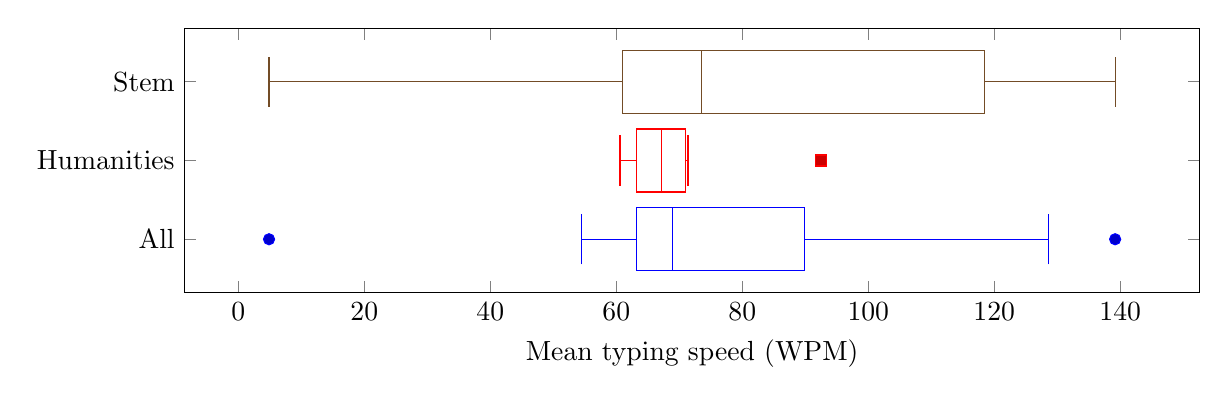
\begin{tikzpicture}
        \begin{axis}[
                y=1cm,
                x=0.08cm,
                ytick={1,2,3},
                yticklabels={All, Humanities, Stem},
                xlabel={Mean typing speed (WPM)},
            ]
            % All
            \addplot+ [
                boxplot prepared={
                    lower whisker=54.41,
                    lower quartile=63.23,
                    median=68.88,
                    upper quartile=89.825,
                    upper whisker=128.65,
                },
            ] table [row sep=\\,y index=0] {
                data\\ 139.19\\ 4.875\\
            };
            % Humanities
            \addplot+ [
                boxplot prepared={
                    lower whisker=60.59,
                    lower quartile=63.23,
                    median=67.203,
                    upper quartile=71.035,
                    upper whisker=71.385,
                },
            ] table [row sep=\\,y index=0] {
                data\\ 92.5\\
            };
            % STEM
            \addplot+ [
                boxplot prepared={
                    lower whisker=4.875,
                    lower quartile=60.955,
                    median=73.54,
                    upper quartile=118.415,
                    upper whisker=139.19,
                },
            ] coordinates {};
        \end{axis}
    \end{tikzpicture}
\end{figure}

% STEM Histogram
\begin{figure}[ht]
    \centering
    \caption{Histogram of STEM typing speeds}
    \label{fig:stemhist}
    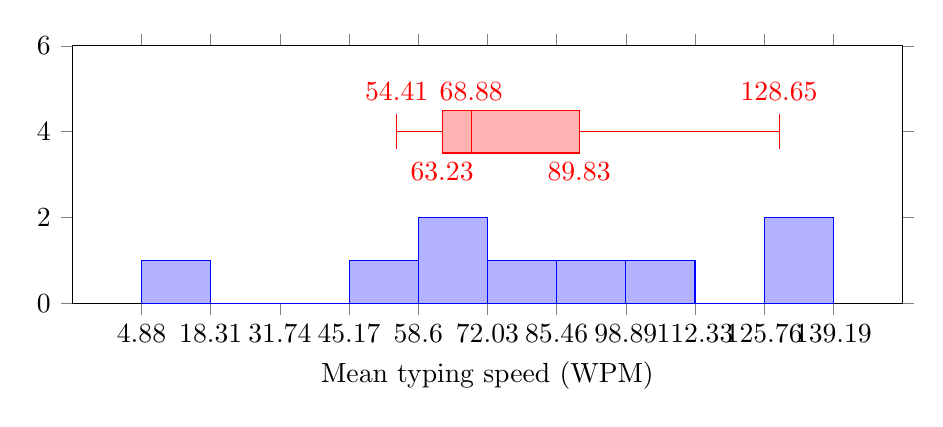
\begin{tikzpicture}
        \begin{axis}[
                width=1\textwidth,
                height=.4\textwidth,
                ymin=0,
                ymax=6,
                xlabel={Mean typing speed (WPM)},
                xtick=data,
                ybar,
                tick align=outside,
            ]
            \addplot+[hist={bins=10}]
            table [row sep=\\,y index=0] {
                data\\
                108.18\\ 54.41\\ 67.5\\ 89.825\\ 139.19\\ 69.87\\ 73.54\\
                128.65\\ 4.875\\
            };
            \addplot+[
                boxplot prepared={
                    draw position=4,
                    box extend=1,
                    lower whisker=54.41,
                    lower quartile=63.23,
                    median=68.88,
                    upper quartile=89.825,
                    upper whisker=128.65,
                },
            ] coordinates {}
            [above]
            node at
                (boxplot box cs: \boxplotvalue{lower whisker},1)
                {\pgfmathprintnumber{\boxplotvalue{lower whisker}}}
            node at
                (boxplot box cs: \boxplotvalue{median},1)
                {\pgfmathprintnumber{\boxplotvalue{median}}}
            node at
                (boxplot box cs: \boxplotvalue{upper whisker},1)
                {\pgfmathprintnumber{\boxplotvalue{upper whisker}}}
            [below]
            node at
                (boxplot box cs: \boxplotvalue{lower quartile},0)
                {\pgfmathprintnumber{\boxplotvalue{lower quartile}}}
            node at
                (boxplot box cs: \boxplotvalue{upper quartile},0)
                {\pgfmathprintnumber{\boxplotvalue{upper quartile}}}
            ;
        \end{axis}
    \end{tikzpicture}
\end{figure}

% Humanities Histogram
\begin{figure}[ht]
    \centering
    \caption{Histogram of Humanities typing speeds}
    \label{fig:stemhist}
    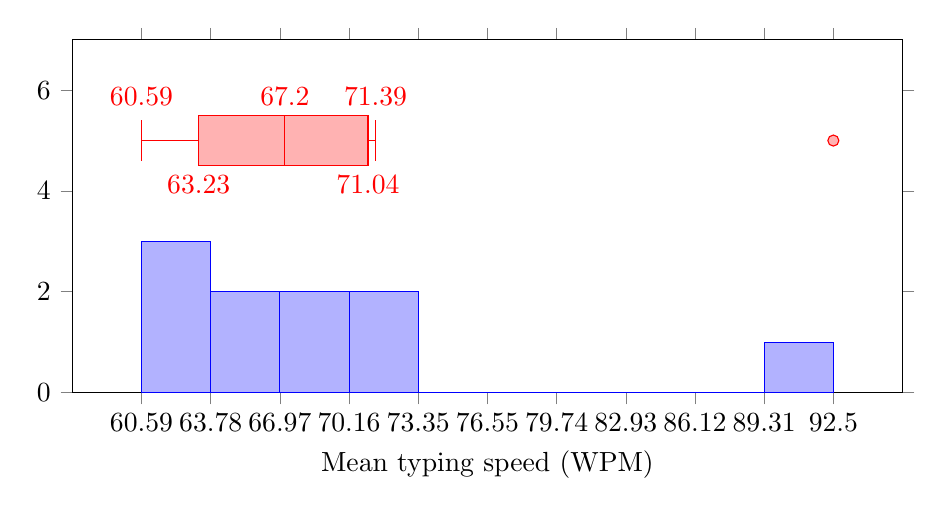
\begin{tikzpicture}
        \begin{axis}[
                width=1\textwidth,
                height=.5\textwidth,
                ymin=0,
                ymax=7,
                xlabel={Mean typing speed (WPM)},
                xtick=data,
                ybar,
                tick align=outside,
            ]
            \addplot+[hist={bins=10}]
            table [row sep=\\,y index=0] {
                data\\
                    60.59\\ 62.545\\ 63.23\\ 67.5\\ 66.905\\ 92.5\\ 71.035\\
                    71.385\\ 65.325\\ 68.88\\
            };
            \addplot+[
                boxplot prepared={
                    draw position=5,
                    box extend=1,
                    lower whisker=60.59,
                    lower quartile=63.23,
                    median=67.203,
                    upper quartile=71.035,
                    upper whisker=71.385,
                },
            ] table [row sep=\\,y index=0] {
                data\\ 92.5\\
            }
            [above]
            node at
                (boxplot box cs: \boxplotvalue{lower whisker},1)
                {\pgfmathprintnumber{\boxplotvalue{lower whisker}}}
            node at
                (boxplot box cs: \boxplotvalue{median},1)
                {\pgfmathprintnumber{\boxplotvalue{median}}}
            node at
                (boxplot box cs: \boxplotvalue{upper whisker},1)
                {\pgfmathprintnumber{\boxplotvalue{upper whisker}}}
            [below]
            node at
                (boxplot box cs: \boxplotvalue{lower quartile},0)
                {\pgfmathprintnumber{\boxplotvalue{lower quartile}}}
            node at
                (boxplot box cs: \boxplotvalue{upper quartile},0)
                {\pgfmathprintnumber{\boxplotvalue{upper quartile}}}
            ;
        \end{axis}
    \end{tikzpicture}
\end{figure}

\newpage

% Summary statistics
\begin{figure}[ht]
    \centering
    \begin{tabular}{lrrr}
        \toprule
        Group & Mean & Median & Standard Deviation \\
        \midrule
        All & 75.049 & 68.88 & 28.708 \\
        Humanities & 68.9895 & 67.203 & 8.993 \\
        STEM & 81.782 & 73.54 & 40.822 \\
    \end{tabular}
    \caption{Summary statistics}
    \label{table:summary}
\end{figure}

\section{Inference, Interpretation, \& Conclusion}

\begin{figure}[ht]
    \centering
    \begin{tabular}{lp{0.5\textwidth}}
        \toprule
        Condition & Satisfied \\
        \midrule
        Random & RCHS seniors were randomly selected \\
        Independence & Speeds from one student shouldn't impact other students' speeds \\
        \bf{Nearly normal} & \bf{Histograms are not nearly normal and $n$ is
        not great enough for central limit theorem to take effect} \\
    \end{tabular}
    \caption{Conditions for inference}
    \label{table:conditions}
\end{figure}

Our test breaks the nearly normal condition required to make inferences on two
sample means. These histograms are not normally distributed and the sample size
of each group is not large enough to use the central limit theorem. It is
reasonable to assume that our populations will be nearly normally distributed
(although a rightward skew could be argued). We will proceed with caution and
the knowledge that conditions have not been met.

\newpage

\begin{figure}[ht]
    \begin{subfigure}[t]{0.4\textwidth}
        \centering
        \begin{tabular}[t]{lrr}
            \toprule
            & Outlier & No outlier \\
            \midrule
            $\overline{STEM} - \overline{Huma}$ & 12.793 & 22.407 \\
            df & 8.699  & 7.953 \\
            $t^{\#}$ & -0.920 & -1.986 \\
            p-value & 0.191 & 0.0413 \\
        \end{tabular}
    \end{subfigure}\hfill%
    \begin{subfigure}[t]{0.5\textwidth}
        Assuming the true mean of humanities students’ typing speeds is equal
        to the true mean of STEM students’ typing speeds and the outlier is
        removed, there is a 4.127\% chance of observing STEM students with a
        mean typing speed 22.406 WPM greater than that of humanities students.
        With a p-value of 0.0413 (less than alpha=0.05), we reject the null
        hypothesis and conclude that, assuming the typing speed populations are
        normally distributed, STEM students have a greater mean typing speed
        than humanities students.
    \end{subfigure}
    \caption{Two sample t-test results}
    \label{table:ttest}
\end{figure}

\section{Critique}

The major flaw in our observational study was breaking the nearly normal
inference condition. In the future, this study could be conducted with a
greater sample size, one that is large enough to satisfy the requirements of
the central limit theorem.

\end{document}

